% cpu/overview.tex
% mainfile: ../perfbook.tex
% SPDX-License-Identifier: CC-BY-SA-3.0

\section{概述}
\label{sec:cpu:Overview}
%
\epigraph{机械同理心：硬件与软件和谐协作。}
	 {Martin Thompson}

如果只是粗略地扫一眼计算机系统的规格表，人们很容易觉得CPU的性能就像在一条平坦赛道上赛跑，
如\cref{fig:cpu:CPU Performance at its Best}所示，
总是跑得最快的选手赢得比赛。

\begin{figure}
\centering
\resizebox{3in}{!}{\includegraphics{cartoons/r-2014-CPU-track-meet}}
\caption{CPU最佳性能表现}
\ContributedBy{fig:cpu:CPU Performance at its Best}{Melissa Broussard}
\end{figure}

虽然确实存在少数针对CPU的benchmark能够接近
\cref{fig:cpu:CPU Performance at its Best}中所示的理想情况，
但典型的程序与其说是赛跑，更不如说是障碍赛。
托\IXr{Moore's Law}的福，过去几十年间CPU的内部架构发生了急剧变化。
以下各节将介绍其中一些架构变化。

\subsection{流水线CPU}
\label{sec:cpu:Pipelined CPUs}

\begin{figure}
\centering
\resizebox{3in}{!}{\includegraphics{cartoons/r-2014-Old-man-and-Brat}}
\caption{新旧CPU}
\ContributedBy{fig:cpu:CPUs Old and New}{Melissa Broussard}
\end{figure}

在1980年代，典型的微处理器在处理下一条指令之前，至少需要取指、解码和执行
三个时钟周期来完成当前指令。
相比之下，1990年代末和2000年代的CPU可以同时处理许多条指令，
使用\emph{流水线}、\emph{超标量}技术、\emph{乱序}指令和数据处理、
\emph{推测执行}等更多技术~\cite{Hennessy2017}来优化指令和数据
在CPU中的流动。
一些核心拥有多个硬件线程，这被称为
\emph{同步多线程}（SMT）或\emph{超线程}
（HT）~\cite{JFennel1973SMT}，
每个硬件线程在软件看来都是一个独立的CPU，至少从功能角度来看是这样。
这些现代硬件特性可以极大地提升性能，
如\cref{fig:cpu:CPUs Old and New}所示。

带有长流水线的CPU要达到最佳性能，需要程序具有高度可预测的控制流。
如果程序的主要代码是在执行紧凑循环，那么就能提供这样的控制流，
例如对大型矩阵或向量进行算术运算的程序。
此时CPU可以正确预测出在大多数情况下循环末尾的分支走向，
从而保持流水线满载，让CPU全速运行。

\begin{figure}
\centering
\resizebox{3in}{!}{\includegraphics{cartoons/r-2014-branch-error}}
\caption{CPU遭遇流水线冲刷}
\ContributedBy{fig:cpu:CPU Meets a Pipeline Flush}{Melissa Broussard}
\end{figure}

然而，分支预测并不总是那么容易。
例如，如果程序中带有许多循环，且每个循环的迭代计数都比较小，
或者面向对象的程序中带有许多虚方法，每个虚方法都可以引用不同的对象实例，
而这些对象实例都实现了一些频繁被调用的成员函数，
此时CPU很难甚至完全不可能预测某个分支的走向。
这样CPU要么等待控制流进行到足以知道分支走向的地步，
要么干脆猜测并使用推测执行继续前进。
虽然猜测对于控制流可预测的程序效果极好，
但对于不可预测的分支（如二分搜索中的分支），
CPU常常猜错。
一次错误的猜测代价很高，因为CPU必须丢弃错误分支之后所有
推测执行的指令，导致流水线冲刷。
如果流水线冲刷发生得过于频繁，就会大幅降低整体性能，
如\cref{fig:cpu:CPU Meets a Pipeline Flush}中所夸张描绘的那样。

\begin{figure}
\centering
\resizebox{3in}{!}{\includegraphics{cpu/microarch}}
\caption{现代微架构概略图}
\label{fig:cpu:Rough View of Modern Micro-Architecture}
\end{figure}

对于超线程（或SMT，如果你更喜欢这个叫法的话）来说情况更糟，
特别是在具有推测执行功能的流水线超标量乱序CPU上。
在这种日益常见的情况下，共享一个核心的所有硬件线程也共享该核心的资源，
包括寄存器、cache、执行单元等等。
指令通常被解码为微操作，共享执行单元和数百个硬件寄存器的使用通常
由一个微操作调度器来协调。
这样一个双线程核心的概略图如
\cref{fig:cpu:Rough View of Modern Micro-Architecture}所示，
更精确（因而也更复杂）的图可以在教科书和学术论文中找到。\footnote{
	这是一个2010年代末的Intel核心的示例：
	\url{https://en.wikichip.org/wiki/intel/microarchitectures/skylake_(server)}。}
因此，一个硬件线程的执行可能而且经常会受到共享同一核心的
其他硬件线程的行为的干扰。

即使只有一个硬件线程处于活动状态（例如，在只有一个线程的
传统CPU设计中），反直觉的结果也相当常见。
执行单元往往具有重叠的功能，因此CPU对执行单元的选择
可能会导致流水线停顿，因为后续指令会争用该执行单元。
理论上这种争用是可以避免的，但实际上CPU必须非常快速地做出选择，
且无法预知未来。
特别值得注意的是，向一个紧密循环中添加一条指令，
有时反而会使执行\emph{加速}。

不幸的是，流水线冲刷和共享资源争用并不是现代CPU在其
障碍赛道上面临的唯一风险。
下一节将介绍内存引用的相关风险。

\subsection{内存引用}
\label{sec:cpu:Memory References}

在1980年代，微处理器从内存读取一个值的时间通常比执行一条指令还短。
而在较近的时期，同样是读取内存里一个值的时间，微处理器可以执行数百甚至数千条指令。
这种差距主要源于\IXr{Moore's Law}使得CPU性能的增长速度大大超过
内存\IX{latency}的降低速度，也有部分来源于内存容量的增长速度。
例如，1970年代的典型小型计算机通常只有4\,KB
（是的，是千字节，不是兆字节，更别提吉字节或太字节了）的主存，
且访问只需一个CPU周期。\footnote{
	公平地说，这些单周期中的每一个周期都不少于1.6\emph{微秒}。}
如今的CPU设计师仍然可以设计出单周期访问的4\,KB内存，
即使在具有多GHz时钟频率的系统上也是如此。
事实上他们确实经常设计这样的内存，只不过现在称之为
``零级cache''，容量也大大超过4\,KB。

\begin{figure}
\centering
\resizebox{3in}{!}{\includegraphics{cartoons/r-2014-memory-reference}}
\caption{CPU遭遇内存引用}
\ContributedBy{fig:cpu:CPU Meets a Memory Reference}{Melissa Broussard}
\end{figure}

虽然现代微处理器上的大容量cache极大地减少了内存访问延迟，
但只有高度可预测的数据访问模式才能让cache发挥最大效用。
不幸的是，像遍历链表这样的常见操作具有极其不可预测的内存访问模式——
毕竟，如果这些模式是可预测的，我们也就不会被指针所困扰了，对吧？
因此，如\cref{fig:cpu:CPU Meets a Memory Reference}所示，
内存引用往往对CPU性能造成严重影响。

到目前为止，我们只考虑了给定CPU在执行单线程代码时可能遇到的障碍。
多线程给CPU带来了额外的障碍，如以下各节所述。

\subsection{原子操作}
\label{sec:cpu:Atomic Operations}

还有一种障碍是\IX{atomic}操作。
原子操作（atomic operation）的概念在某种意义上与CPU流水线一次执行多条指令的
运作方式相冲突。
拜硬件设计者的精密设计所赐，现代CPU使用了许多极其巧妙的技巧使这些操作
\emph{看起来}是原子的，尽管它们实际上是逐步执行的。
一个常见的技巧是：标出所有包含原子操作所需数据的cache line，
确保CPU在执行原子操作时这些cache line都归该CPU所有，
并且只有在这些cache line仍归该CPU所有时才推进原子操作的执行。
这样一来，因为所有数据都只属于该CPU，即使CPU的流水线可以同时执行多条指令，
其他CPU也无法干扰此CPU的原子操作执行。
不用多说，这种技巧要求流水线必须能被延迟甚至冲刷，
才能执行让原子操作正确完成的一系列准备操作。

\begin{figure}
\centering
\resizebox{3in}{!}{\includegraphics{cartoons/r-2014-Atomic-reference}}
\caption{CPU遭遇原子操作}
\ContributedBy{fig:cpu:CPU Meets an Atomic Operation}{Melissa Broussard}
\end{figure}

非原子操作则与之相反，CPU可以从cache line中按照数据到达的顺序加载值，
并将结果放入store buffer中，无需等待cache line的所有权切换。
虽然有一些硬件优化有时可以隐藏cache延迟，
但原子操作对性能的影响往往如
\cref{fig:cpu:CPU Meets an Atomic Operation}所描绘的那样。

不幸的是，原子操作通常只适用于单个数据元素。
由于许多并行算法要求在多个数据元素的更新之间维持排序约束，
大多数CPU提供了memory barrier。
这些memory barrier也是性能消耗的障碍，如下一节所述。

\QuickQuiz{
	什么类型的机器能够对多个数据元素执行原子操作？
}\QuickQuizAnswer{
	一个答案是，通常可以将多个数据元素打包到一个机器字中，
	然后对其进行原子操作。

	一个更时髦的答案是支持事务内存（transactional memory）的
	机器~\cite{DBLomet1977SIGSOFT,Knight:1986:AMF:319838.319854,Herlihy93a}。
	到2014年初，几个主流系统提供了有限的硬件事务内存实现，
	其优缺点在\cref{sec:future:Hardware Transactional Memory}中有更详细的介绍。
	关于软件事务内存的适用性，业界也尚未定论~\cite{McKenney2007PLOSTM,DonaldEPorter2007TRANSACT,
	ChistopherJRossbach2007a,CalinCascaval2008tmtoy,
	AleksandarDragovejic2011STMnotToy,AlexanderMatveev2012PessimisticTM}，
	相关内容在\cref{sec:future:Transactional Memory}中有所介绍。
}\QuickQuizEnd

\subsection{内存屏障（memory barrier）}
\label{sec:cpu:Memory Barriers}

\IXpl{Memory barrier}将在
\cref{chp:Advanced Synchronization: Memory Ordering}和
\cref{chp:app:whymb:Why Memory Barriers?}中更详细地讨论\@。
在此期间，考虑以下简单的基于lock的\IX{critical
section}：

\begin{VerbatimN}[samepage=true]
spin_lock(&mylock);
a = a + 1;
spin_unlock(&mylock);
\end{VerbatimN}

\begin{figure}
\centering
\resizebox{3in}{!}{\includegraphics{cartoons/r-2023-Memory-barrier}}
\caption{CPU遭遇Memory Barrier}
\ContributedBy{fig:cpu:CPU Meets a Memory Barrier}{Melissa Broussard}
\end{figure}

如果CPU没有按照上述语句的顺序执行，
变量``a''就会在没有``mylock''保护的情况下被递增，
这肯定和我们获取锁的目的不一致。
为了防止这种有害的乱序执行，锁操作原语中必须包含显式或隐式的memory barrier。
由于memory barrier的作用就是阻止CPU（更不用说编译器）
为了提高性能而进行的乱序执行，
所以memory barrier几乎总是会降低性能，
如\cref{fig:cpu:CPU Meets a Memory Barrier}所描绘的那样。

与原子操作一样，CPU设计师一直在努力降低\IXh{memory-barrier}{overhead}，
并已取得了实质性进展。

\subsection{功能单元的不足}
\label{sec:cpu:Functional Unit Failings}

现代超标量CPU拥有众多用途和能力各异的功能单元。
每个CPU可能有多个用于整数和布尔运算的算术逻辑单元（ALU）、
几个向量单元、几个浮点单元（FPU），以及至少各一个的分支单元、
加载单元和存储单元。
不同的CPU当然会有不同的功能单元组合。
然而，不仅不同的应用程序需要不同的功能单元组合，
给定的应用程序在不同的执行阶段也可能需要不同的组合。

\begin{figure}
\centering
\resizebox{2.5in}{!}{\includegraphics{cartoons/CPU-track-meet-functional-units}}
\caption{CPU功能单元不匹配}
\ContributedBy{fig:cpu:CPU Functional-Unit Mismatch}{Melissa Broussard, remixed}
\end{figure}

这意味着，认为某个CPU拥有完美的功能单元组合并没有太大意义。
有时候CPU反而必须``单脚跳着走''，只使用其令人印象深刻的功能单元
阵列中的极少数几个，
如\cref{fig:cpu:CPU Functional-Unit Mismatch}中输掉比赛的
那个不幸的CPU所夸张描绘的那样。

\QuickQuiz{
	但这与在多核CPU上扩展工作负载有什么关系？
}\QuickQuizAnswer{
	在很多情况下，关系相当大！
	例如，在具有超线程核心的系统上，共享一个核心的硬件线程也共享
	其功能单元，这可能导致另一种形式的争用，从而限制可扩展性。
	再举一个例子，拥有令人印象深刻的功能单元阵列的全部意义在于
	支持指令级并行，即CPU内部的并发性和可扩展性。
}\QuickQuizEnd

不幸的是，即使一个工作负载能完美高效地使用给定CPU的每一个功能单元，
它仍然可能失败，例如下一节所描述的情况。

\subsection{热节流}
\label{sec:cpu:Thermal Throttling}

一种越来越常见的令人沮丧的经历是：精心微优化一段关键代码路径，
大幅减少了该代码路径消耗的时钟周期数，
却发现该代码消耗的挂钟时间实际上\emph{增加}了。

\begin{figure}
\centering
\resizebox{3in}{!}{\includegraphics{cartoons/r-2022-Thermal-throttling}}
\caption{CPU遭遇热节流}
\ContributedBy{fig:cpu:Encounters Thermal Throttling}{Melissa Broussard, remixed}
\end{figure}

欢迎来到现代\IX{thermal throttling}的世界。

如果你通过更高效地利用CPU的功能单元来减少时钟周期数，
你就会增加该CPU消耗的功率。
这反过来会增加该CPU散发的热量。
如果这些热量超出了散热系统的能力，系统就会对该CPU进行热节流，
例如降低其时钟频率，
如\cref{fig:cpu:Encounters Thermal Throttling}中的雪企鹅
所夸张描绘的那样。

如果性能至关重要，正确的修复方法是改善散热，
这种方法受到硬核玩家、超频爱好者
（其中一些人善于利用液氮）以及性能优先的系统供应商
（其中有一家使用每CPU一个铝制散热器，每个重达一磅，即0.454公斤）的青睐。
但如果你无法修改计算机的散热系统，
例如因为你是从云服务提供商租用的，
那么你就需要采取其他优化方法。
例如，你可能需要应用算法优化而非以硬件为中心的微优化。
或者，你可以将代码并行化，将工作（因而也是热量）分散到多个CPU核心上。

有些人建议根据各种CPU核心时钟频率来归一化给定测试的结果，
这可能有所帮助。
然而，cache miss和内存访问的延迟并不依赖于CPU核心时钟频率。
此外，如果被测代码涉及多个CPU之间的紧密交互，
那么在一个CPU上运行的代码的性能将取决于其他CPU的核心时钟频率。

最后，如果目标是获得可重复的benchmark测量结果，
一种方法是将传统的cache预热扩展为包括热预热，
所需的预热时间取决于被测系统的大小，因而也取决于其热惯性。

另一种可重复benchmark的方法适用于基于事件的应用程序，
这些程序以短暂但间隔很大的突发形式运行对延迟敏感的执行。
在这种情况下，前述方法的热预热间隔应替换为冷却间隔，
在此期间系统保持空闲。

即使经过了仔细的热预热或冷却，结果仍可能随环境温度的变化而变化，
而环境温度可能强烈依赖于一天中的时段，
更不用说世界某些地区的季节了。

\QuickQuiz{
	在热预热或冷却时间较长且工作负载固定的情况下，
	为什么环境温度会有影响？
}\QuickQuizAnswer{
	是的，以固定CPU核心时钟频率运行的固定工作负载
	确实可能产生恒定的热流，
	尽管在创建CPU热模型时面临许多挑战。
	然而，环境温度越低，热量从CPU流向周围环境的速度就越快。
	这反过来，加上恒定的热流，意味着较低的环境温度将导致较低的CPU温度，
	从而减少热节流。
	因此，给定的benchmark在夜间或冬季可能会产生更高的性能，
	也就是环境温度趋于较低的时候。
}\QuickQuizEnd

\subsection{缓存未命中（cache miss）}
\label{sec:cpu:Cache Misses}

对多线程程序来说，还有一个额外的障碍影响CPU性能——``cache miss''。
正如前文提到的，现代CPU使用大容量cache来降低由于较高的内存访问延迟带来的性能损失。
但是，对于在多个CPU间频繁共享的变量，cache事实上起到了反效果。
因为当某个CPU想去修改该变量时，极有可能该变量的值刚被其他CPU修改过。
在这种情况下，该变量存在于其他CPU而不是当前CPU的cache中，
这将导致代价高昂的cache miss
（更多细节参见\cref{sec:app:whymb:Cache Structure}）。
这种cache miss是CPU性能的主要障碍，
如\cref{fig:cpu:CPU Meets a Cache Miss}所示。

\QuickQuiz{
	那么CPU设计师是否也大幅降低了cache miss的开销？
}\QuickQuizAnswer{
	不幸的是，改善不大。
	在CPU数量不变的情况下有一些降低，
	但有限的光速和物质的原子性质限制了他们
	为更大系统降低cache miss开销的能力。
	\Cref{sec:cpu:Hardware Free Lunch?}
	讨论了未来可能取得进展的一些途径。
}\QuickQuizEnd

\begin{figure}
\centering
\resizebox{3in}{!}{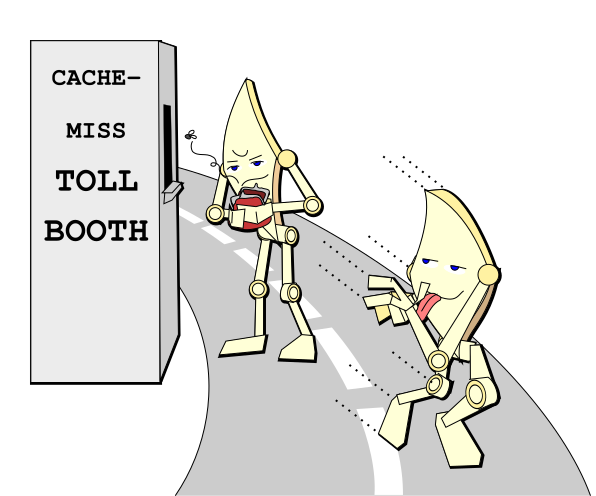
\includegraphics{cartoons/r-2014-CPU-track-meet-cache-miss-toll-booth}}
\caption{CPU遭遇Cache Miss}
\ContributedBy{fig:cpu:CPU Meets a Cache Miss}{Melissa Broussard}
\end{figure}

\subsection{I/O操作}
\label{sec:cpu:I/O Operations}

\begin{figure}
\centering
\resizebox{3in}{!}{\includegraphics{cartoons/r-2014-CPU-track-meet-phone-booth}}
\caption{CPU等待I/O完成}
\ContributedBy{fig:cpu:CPU Waits for I/O Completion}{Melissa Broussard}
\end{figure}

Cache miss可以视为CPU之间的I/O操作，
这应该是代价最低廉的I/O操作之一。
涉及网络、大容量存储器或（更糟的是）人类本身的I/O操作，
对性能的影响远远大于前几节提到的各种障碍，
如\cref{fig:cpu:CPU Waits for I/O Completion}所示。

这也是共享内存式的并行计算和分布式系统式的并行编程的一个不同点：
共享内存式并行编程的程序一般不会处理比cache miss更糟的情况，
而分布式并行编程的程序则很可能遭遇网络通信延迟。
这两种情况的延迟都可看作通信的开销——在顺序程序中所没有的开销。
因此，通信开销占实际执行工作量的比率是一项关键的设计参数。
并行硬件设计的一个主要目标是尽可能降低这个比率，
以达到性能和可扩展性上的目标。
反过来，正如将在\cref{chp:Partitioning and Synchronization Design}中看到的，
并行软件设计的一个主要目标是降低像cache miss这样的
昂贵操作的发生频率。

当然，说某个操作属于性能障碍是一方面，
说某个操作属于对性能影响非常\emph{显著}的障碍则是另一方面。
这一区别将在以下各节中讨论。
